\documentclass[tikz,border=8pt]{standalone}
\usepackage[T1]{fontenc}
\usepackage{helvet}
\renewcommand{\familydefault}{\sfdefault}
\usepackage{graphicx}
\usepackage{xcolor}
\usepackage{tikz}
\usetikzlibrary{arrows.meta,backgrounds,calc,fit,positioning,shapes.geometric}

\definecolor{sgnavy}{HTML}{173B72}
\definecolor{sgblue}{HTML}{2E6DB4}
\definecolor{sgteal}{HTML}{25A7A1}
\definecolor{sgred}{HTML}{E63B47}
\definecolor{sgorange}{HTML}{F28C28}
\definecolor{sggreen}{HTML}{4D9460}
\definecolor{sggray}{HTML}{5F6B76}
\definecolor{sglight}{HTML}{F2F5F8}
\definecolor{sgline}{HTML}{CBD5DF}

\tikzset{
  box/.style={
    draw=sgline,
    fill=white,
    rounded corners=2pt,
    line width=.7pt,
    minimum height=13mm,
    text width=28mm,
    align=center,
    inner sep=3mm,
    font=\small
  },
  compactbox/.style={
    draw=sgline,
    fill=white,
    rounded corners=2pt,
    line width=.7pt,
    minimum height=10mm,
    text width=23mm,
    align=center,
    inner sep=2mm,
    font=\scriptsize
  },
  sourcebox/.style={
    box,
    draw=sgblue,
    fill=sgblue!5
  },
  servicebox/.style={
    box,
    draw=sgteal,
    fill=sgteal!5
  },
  databox/.style={
    box,
    draw=sggreen,
    fill=sggreen!6
  },
  decisionbox/.style={
    diamond,
    draw=sgnavy,
    fill=white,
    aspect=2.4,
    align=center,
    inner sep=1.8mm,
    font=\scriptsize
  },
  layerbox/.style={
    draw=sgline,
    fill=sglight,
    rounded corners=3pt,
    inner sep=5mm
  },
  flow/.style={
    -{Latex[length=2.5mm]},
    line width=1pt,
    draw=sgnavy
  },
  dataflow/.style={
    -{Latex[length=2.5mm]},
    line width=1pt,
    draw=sgteal
  },
  warningflow/.style={
    -{Latex[length=2.5mm]},
    line width=1pt,
    draw=sgred
  },
  labeltext/.style={font=\scriptsize, text=sggray, align=center, fill=white, inner sep=1.5pt},
  zonelabel/.style={font=\bfseries\scriptsize, text=sgnavy, fill=sglight, inner sep=1pt},
  titletext/.style={font=\bfseries\large, text=sgnavy}
}

\begin{document}
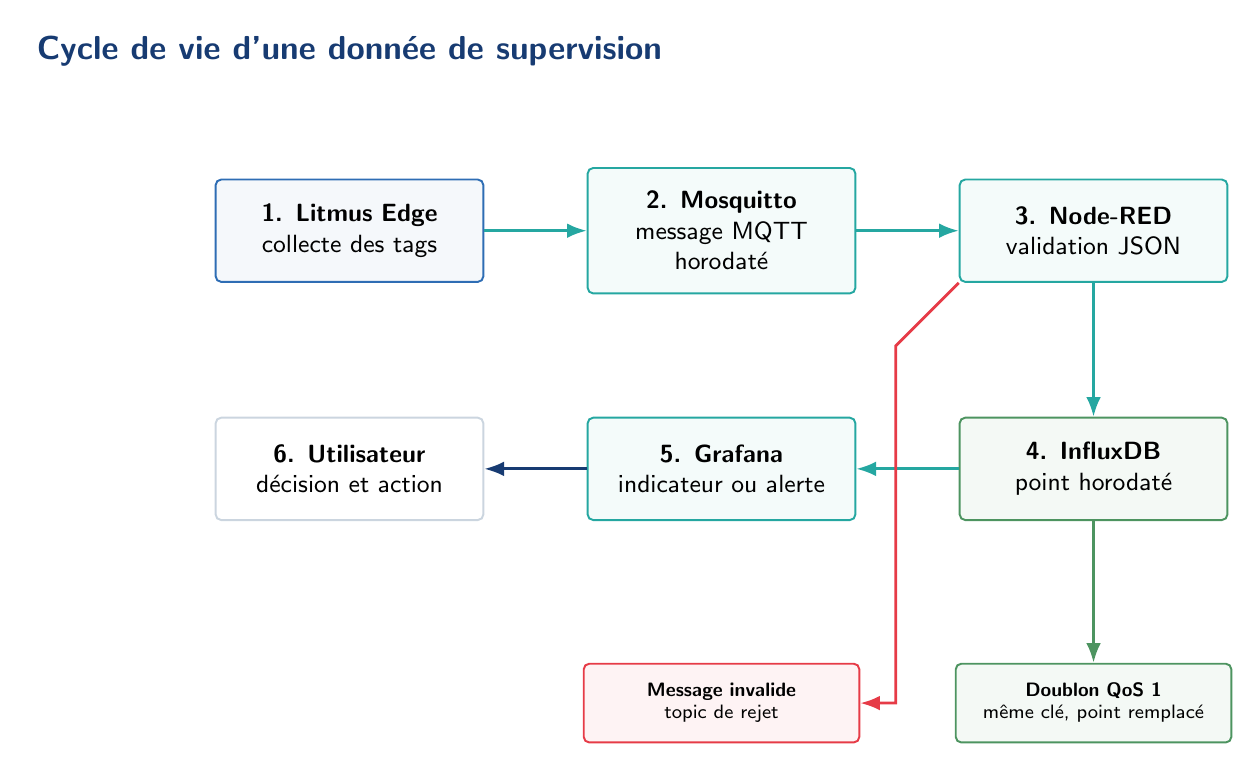
\begin{tikzpicture}[node distance=11mm and 13mm]
  \node[titletext] (title) {Cycle de vie d'une donnée de supervision};

  \node[sourcebox, below=13mm of title, text width=28mm] (litmus)
    {\textbf{1. Litmus Edge}\\collecte des tags};
  \node[servicebox, right=of litmus, text width=28mm] (publish)
    {\textbf{2. Mosquitto}\\message MQTT horodaté};
  \node[servicebox, right=of publish, text width=28mm] (validate)
    {\textbf{3. Node-RED}\\validation JSON};

  \node[databox, below=17mm of validate, text width=28mm] (store)
    {\textbf{4. InfluxDB}\\point horodaté};
  \node[servicebox, left=of store, text width=28mm] (use)
    {\textbf{5. Grafana}\\indicateur ou alerte};
  \node[box, left=of use, text width=28mm] (human)
    {\textbf{6. Utilisateur}\\décision et action};

  \draw[dataflow] (litmus) -- (publish);
  \draw[dataflow] (publish) -- (validate);
  \draw[dataflow] (validate) -- (store);
  \draw[dataflow] (store) -- (use);
  \draw[flow] (use) -- (human);

  \node[compactbox, below=18mm of use, draw=sgred, fill=sgred!6,
        text width=31mm] (reject)
    {\textbf{Message invalide}\\topic de rejet};
  \draw[warningflow] (validate.south west) -- ++(-8mm,-8mm) |- (reject.east);

  \node[compactbox, below=18mm of store, draw=sggreen, fill=sggreen!6,
        text width=31mm] (dedup)
    {\textbf{Doublon QoS 1}\\même clé, point remplacé};
  \draw[flow, draw=sggreen] (store) -- (dedup);
\end{tikzpicture}
\end{document}
